\documentclass[10pt]{standalone}
\usepackage[utf8]{inputenc}
\usepackage{pgf,tikz,pgfplots}
\pgfplotsset{compat=1.15}
\usepackage{mathrsfs}
\usetikzlibrary{arrows}
\pagestyle{empty}
\begin{document}
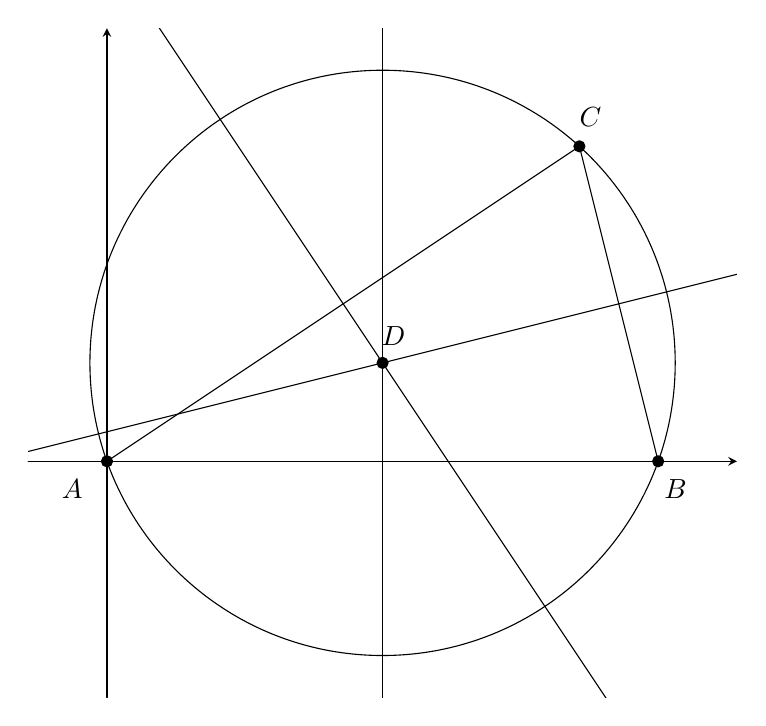
\begin{tikzpicture}[line cap=round,line join=round,>=triangle 45,x=1.0cm,y=1.0cm]
\begin{axis}[
x=1.0cm,y=1.0cm,
axis lines=middle,
ticks=none,
xmin=-1.0,
xmax=8.0,
ymin=-3.0,
ymax=5.5,]
\clip(-1.,-3.) rectangle (8.,5.5);
%\fill[color=black,fill=black,fill opacity=0.1] (0.,0.) -- (7.,0.) -- (6.,4.) -- cycle;
\draw  (0.,0.)-- (7.,0.);
\draw  (7.,0.)-- (6.,4.);
\draw  (6.,4.)-- (0.,0.);
\draw  (3.5, 1.25) circle [radius=3.7165171868296265cm];
\draw  (3.5,-3.) -- (3.5,5.5);
\draw [domain=-1.:8.] plot(\x,{(--26.-6.*\x)/4.});
\draw [domain=-1.:8.] plot(\x,{(-1.5-1.*\x)/-4.});
\begin{scriptsize}
\draw [fill=black] (0.,0.) circle [radius=2.0pt];
\draw (-0.44,-0.35) node {$A$};
\draw [fill=black] (7.,0.) circle [radius=2.0pt];
\draw (7.22,-0.35) node {$B$};
\draw [fill=black] (6.,4.) circle [radius=2.0pt];
\draw (6.14,4.37) node {$C$};

\draw [fill=black] (3.5,1.25) circle [radius=2.0pt];
\draw (3.64,1.59) node {$D$};
\end{scriptsize}
\end{axis}
\end{tikzpicture}
\end{document}